% !TeX root = diploma.tex

\begin{figure}[p]\label{fig:gpinit}
\centering
\subfloat[]{
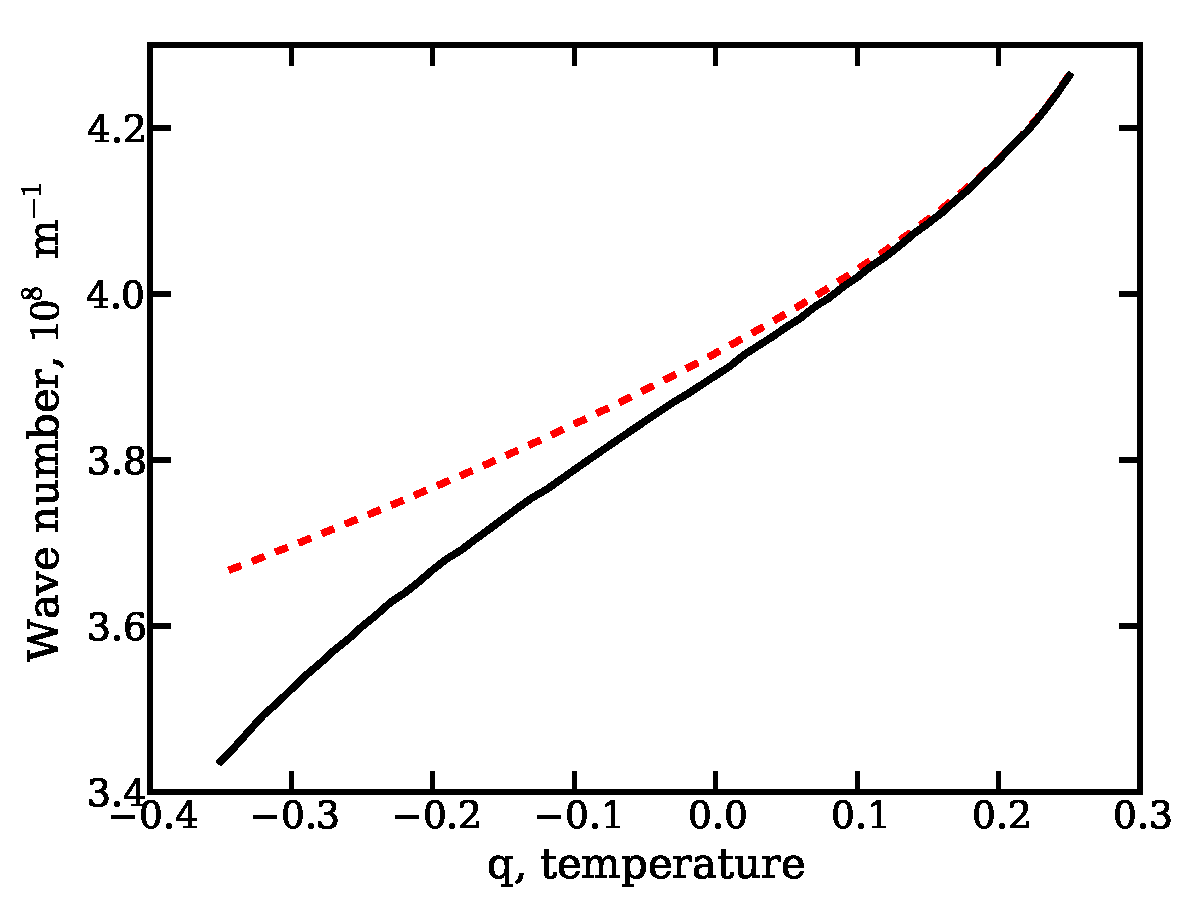
\includegraphics[width = 0.5\textwidth]{figs/gpinit-wn.pdf}
\label{fig:gpinit-wn}}
\subfloat[]{
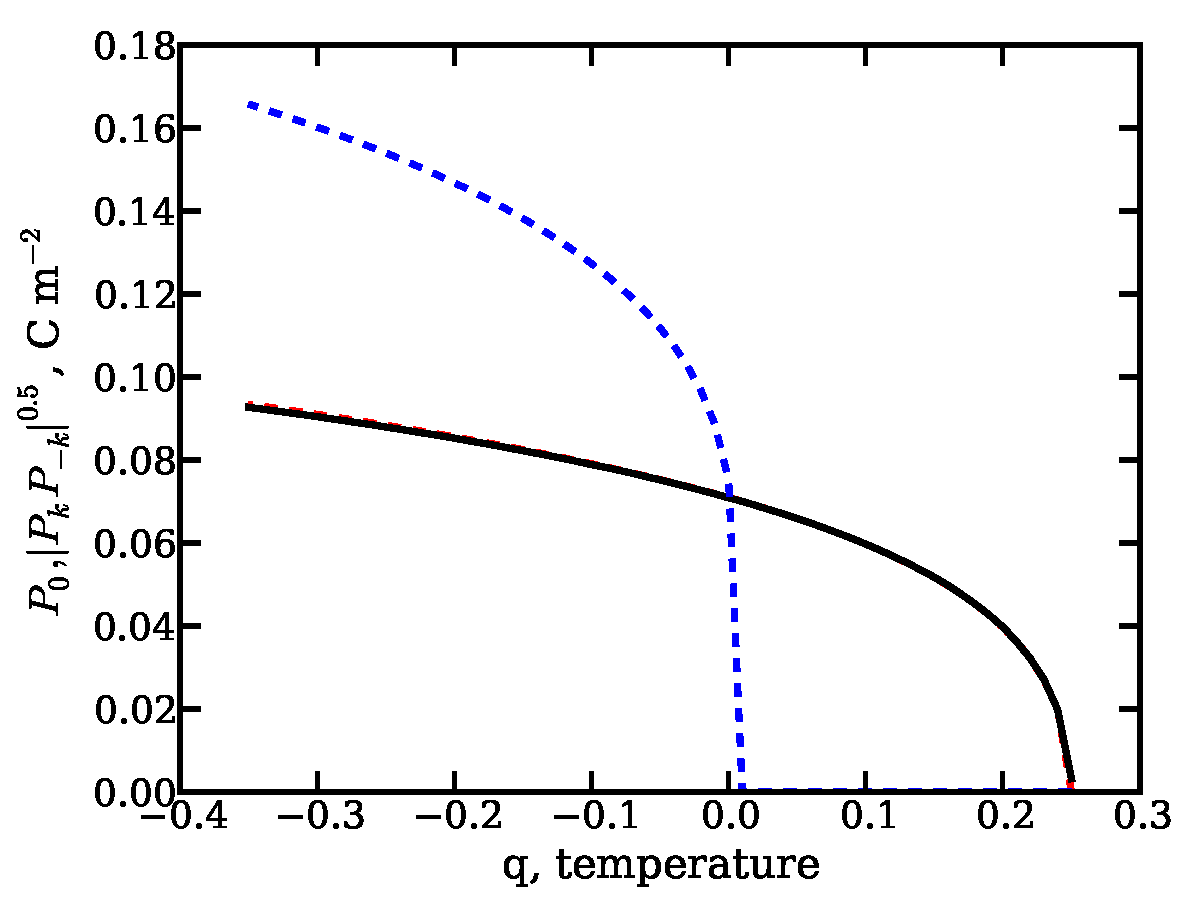
\includegraphics[width = 0.5\textwidth]{figs/gpinit-a.pdf}
\label{fig:gpinit-a}}
\newline
\subfloat[]{
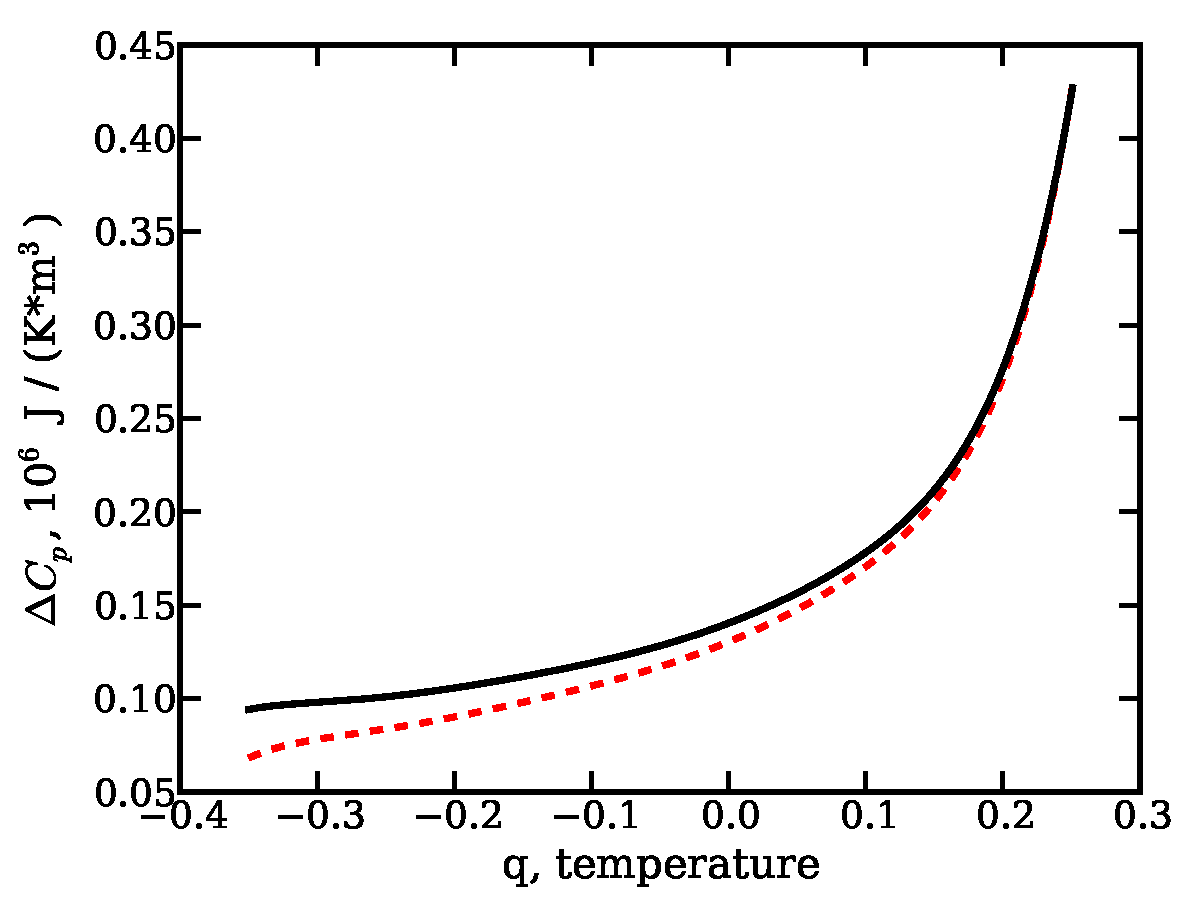
\includegraphics[width = 0.5\textwidth]{figs/gpinit-cp.pdf}
\label{fig:gpinit-cp}}
\newline
\caption{Результаты вычислений для $g= -1.241$, $p_{icp}= -0.088$, $p_{cp}=-0.137$:
\newline \protect\subref{fig:gpinit-wn} для волнового числа; 
\newline \protect\subref{fig:gpinit-a} для амплитуды ПП;
\newline \protect\subref{fig:gpinit-cp} для скачка теплоемкости, отнесенного к температуре.}
\end{figure}

\begin{figure}[p]\label{fig:nogap}
\centering
\subfloat[]{
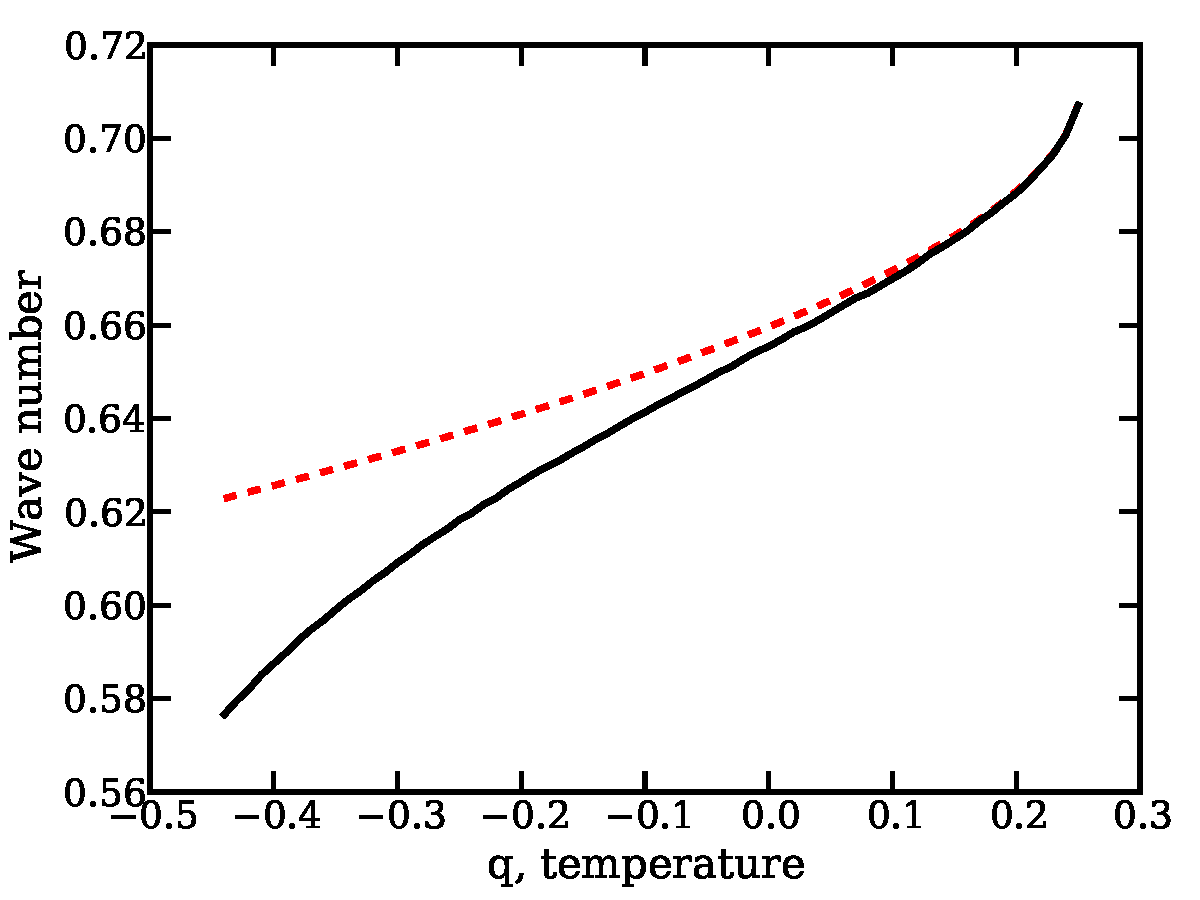
\includegraphics[width = 0.5\textwidth]{figs/nogap-wn.pdf}
\label{fig:nogap-wn}}
\subfloat[]{
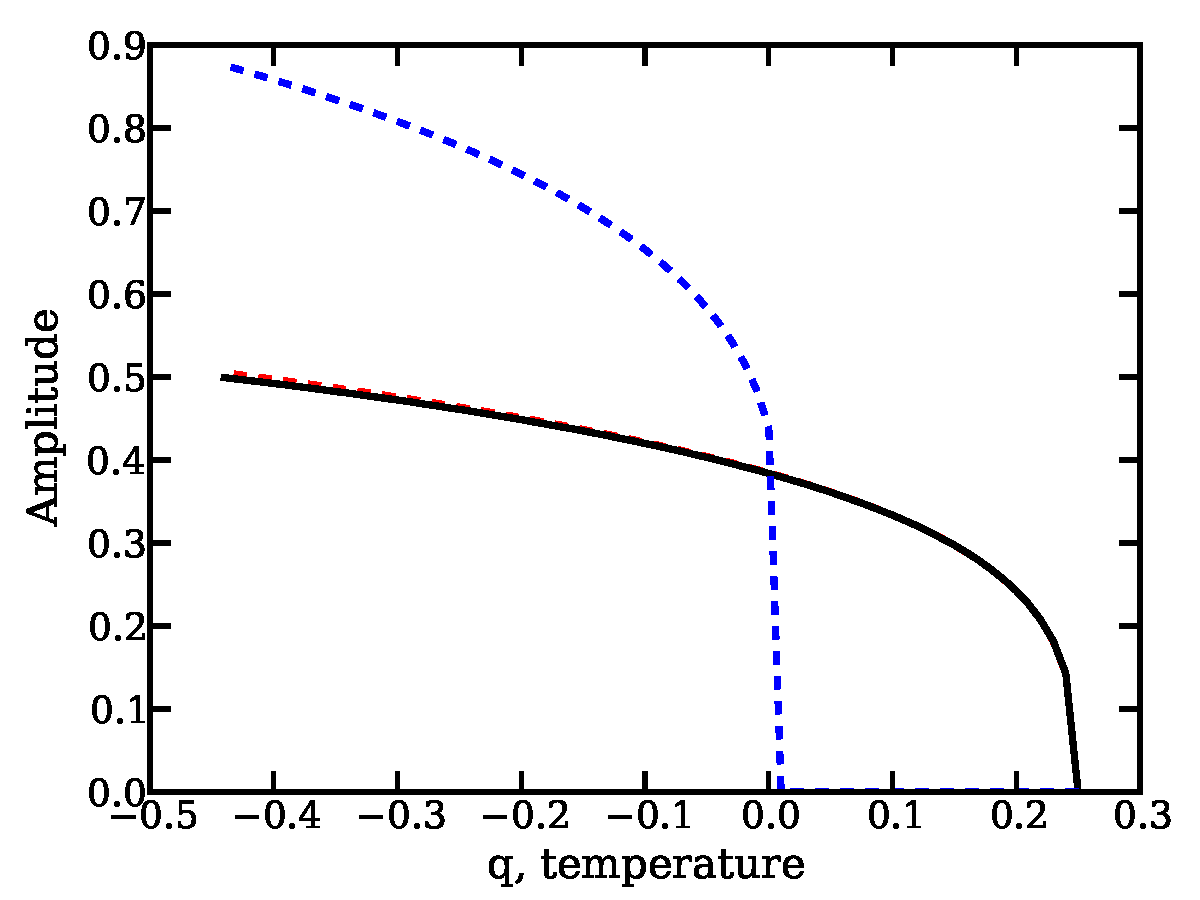
\includegraphics[width = 0.5\textwidth]{figs/nogap-a.pdf}
\label{fig:nogap-a}}
\newline
\subfloat[]{
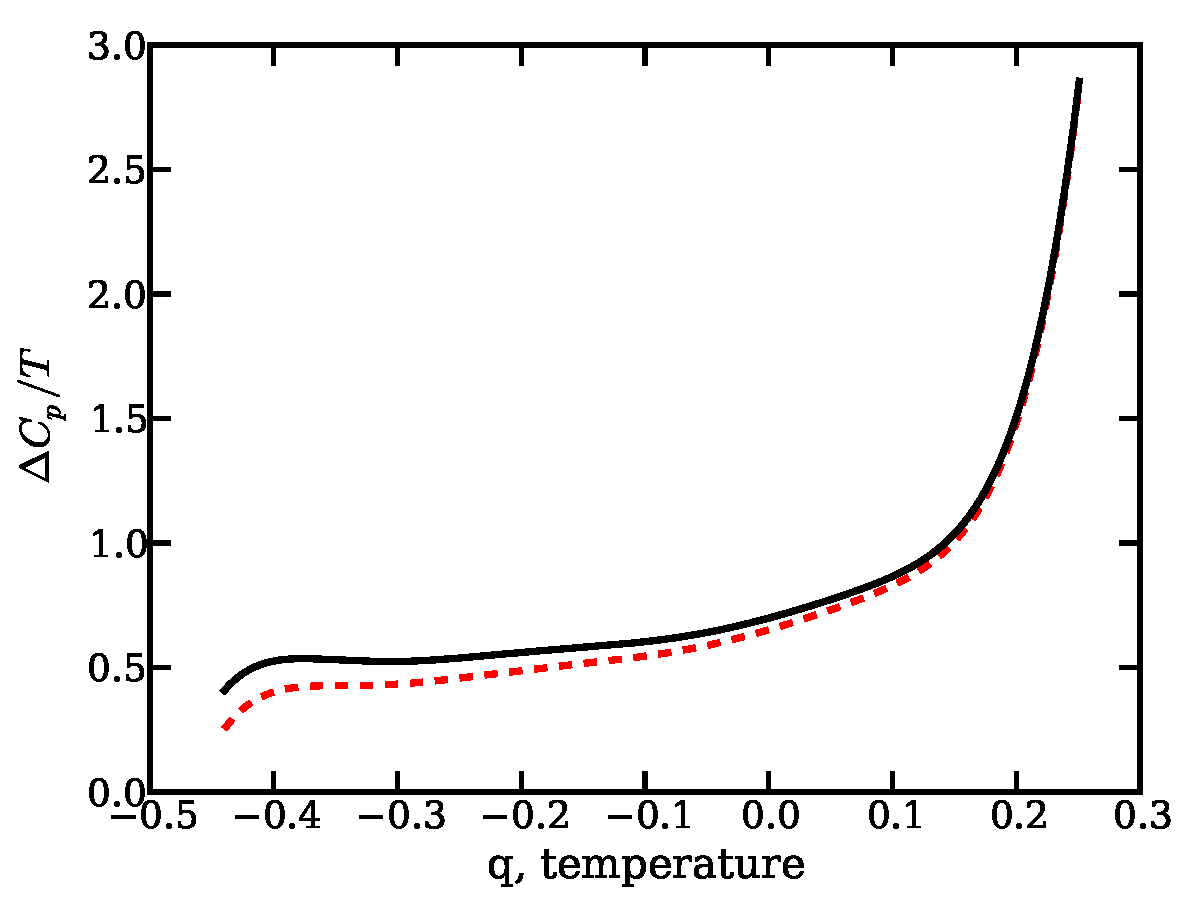
\includegraphics[width = 0.5\textwidth]{figs/nogap-cpt.pdf}
\label{fig:nogap-cpt}}
\newline
\caption{Результаты вычислений для $g= -1.241$, $p_{icp}=p_{cp}=-0.137$ (энергетическая щель отсутствует).}
\end{figure}

\begin{figure}[p]\label{fig:gx3}
\centering
\subfloat[]{
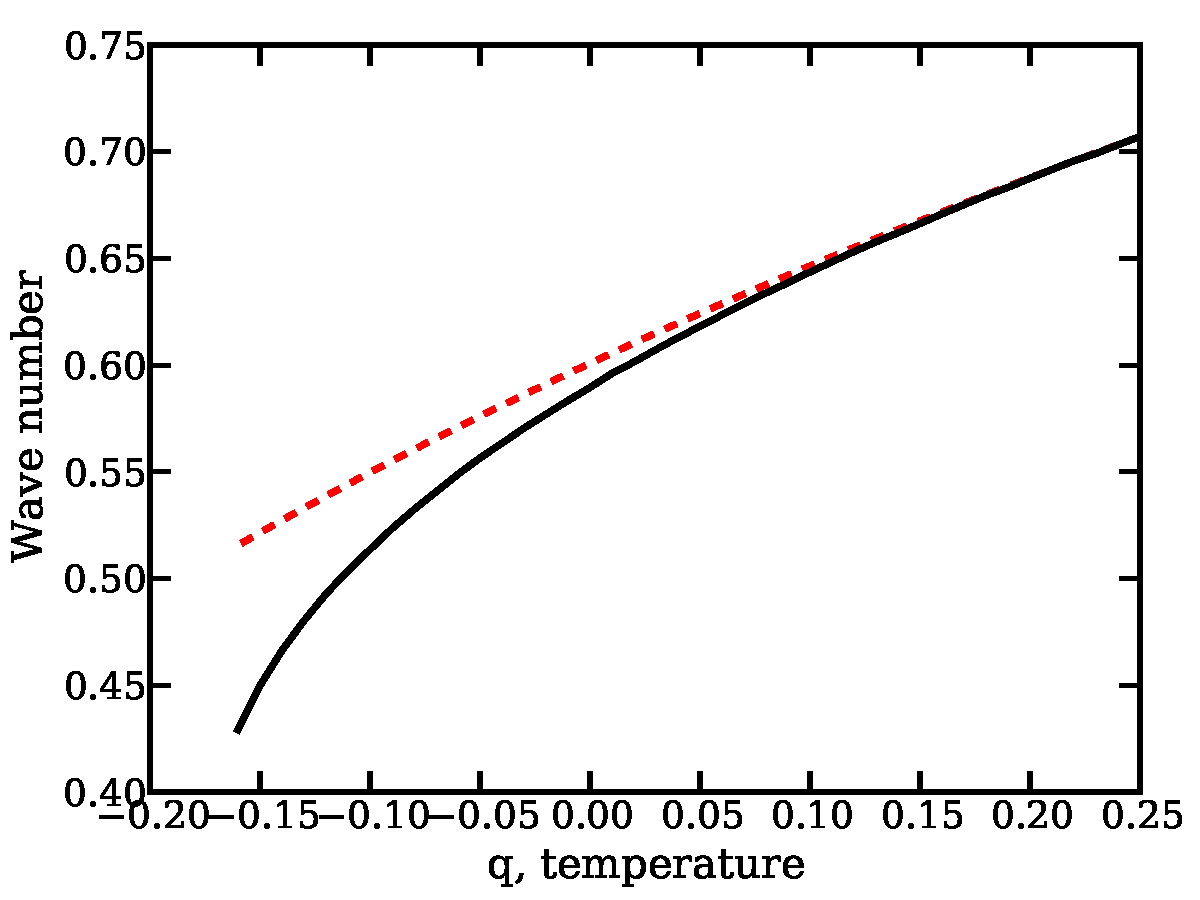
\includegraphics[width = 0.5\textwidth]{figs/gx3-wn.pdf}
\label{fig:gx3-wn}}
\subfloat[]{
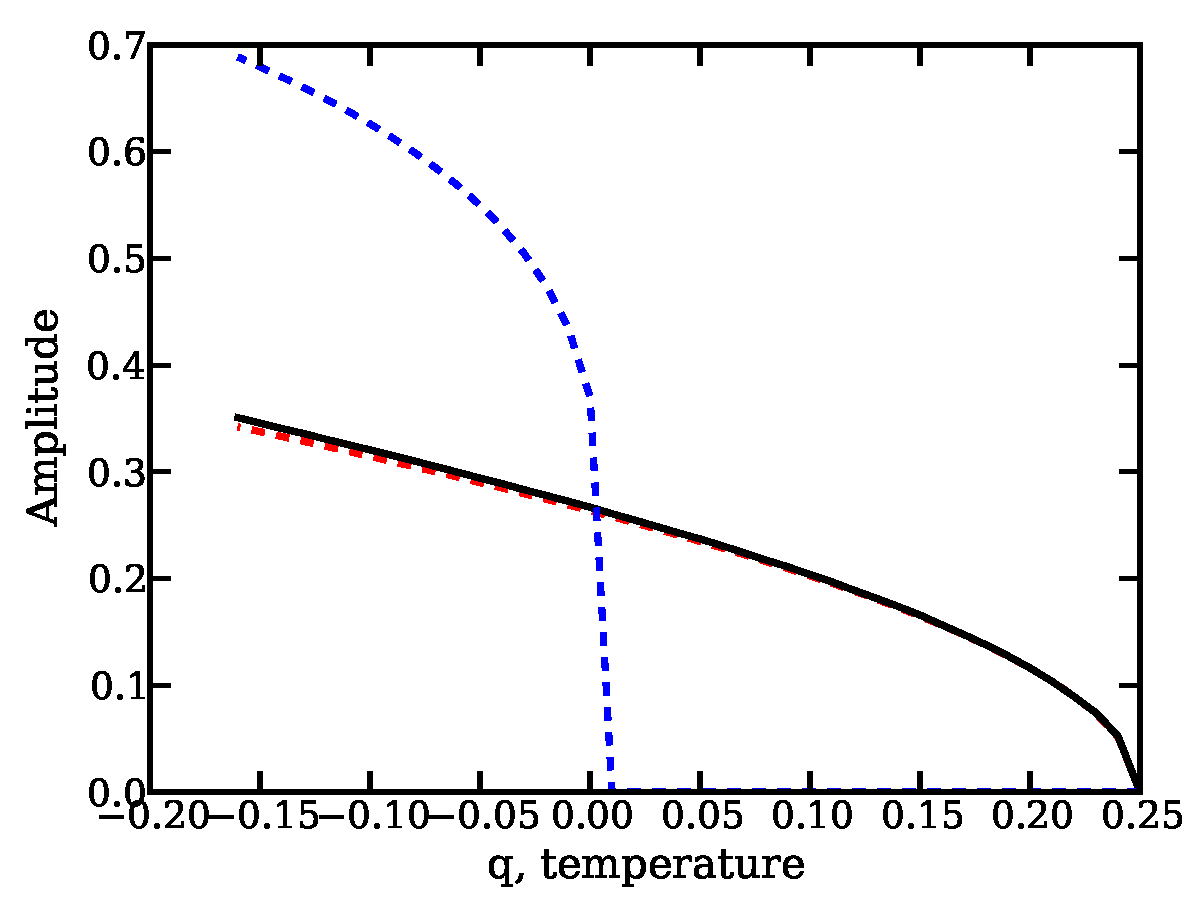
\includegraphics[width = 0.5\textwidth]{figs/gx3-a.pdf}
\label{fig:gx3-a}}
\newline
\subfloat[]{
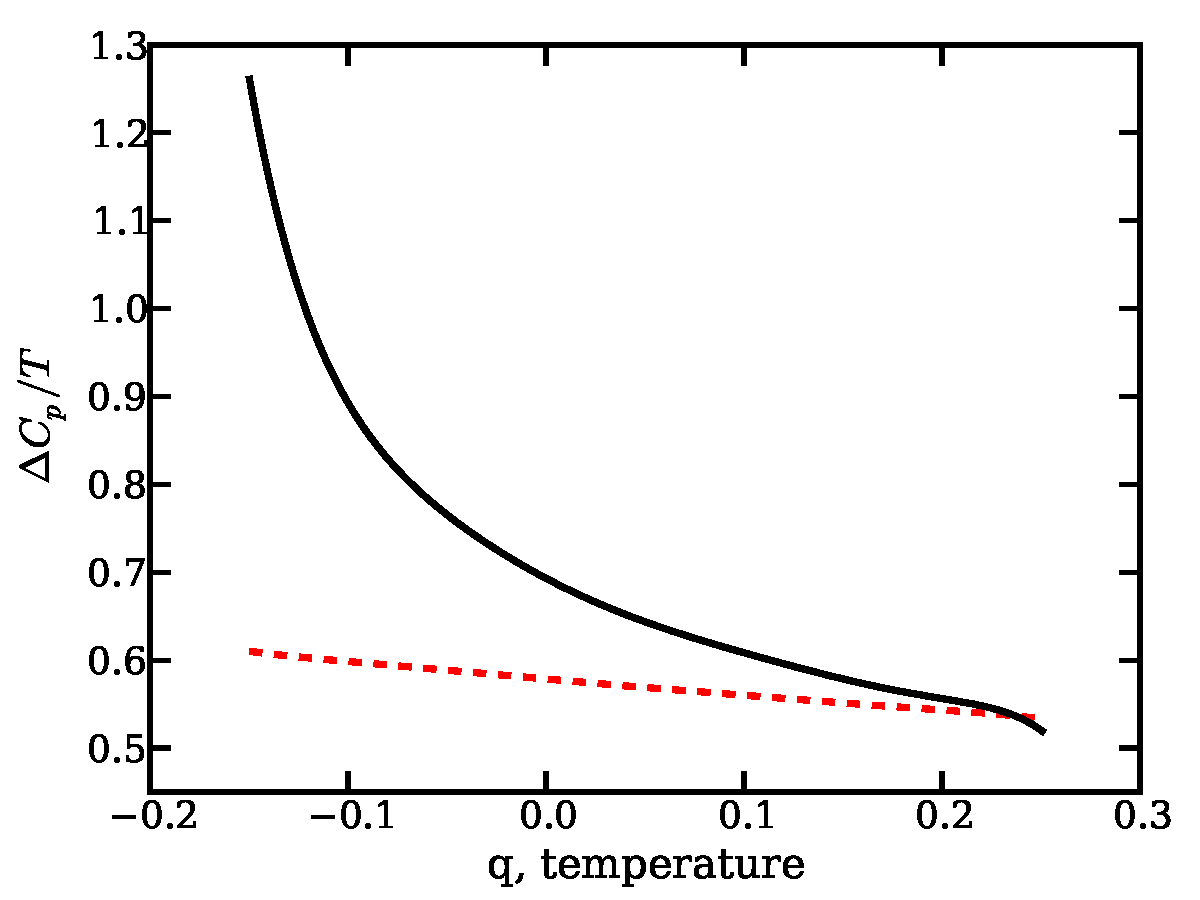
\includegraphics[width = 0.5\textwidth]{figs/gx3-cpt.pdf}
\label{fig:gx3-cpt}}
\newline
\caption{Результаты вычислений для $g= -3.723$, $p_{icp}= -0.088$, $p_{cp}=-0.137$ ($g$ увеличено в 3 раза).}
\end{figure}

\begin{figure}\label{fig:gx3p!3-wn}
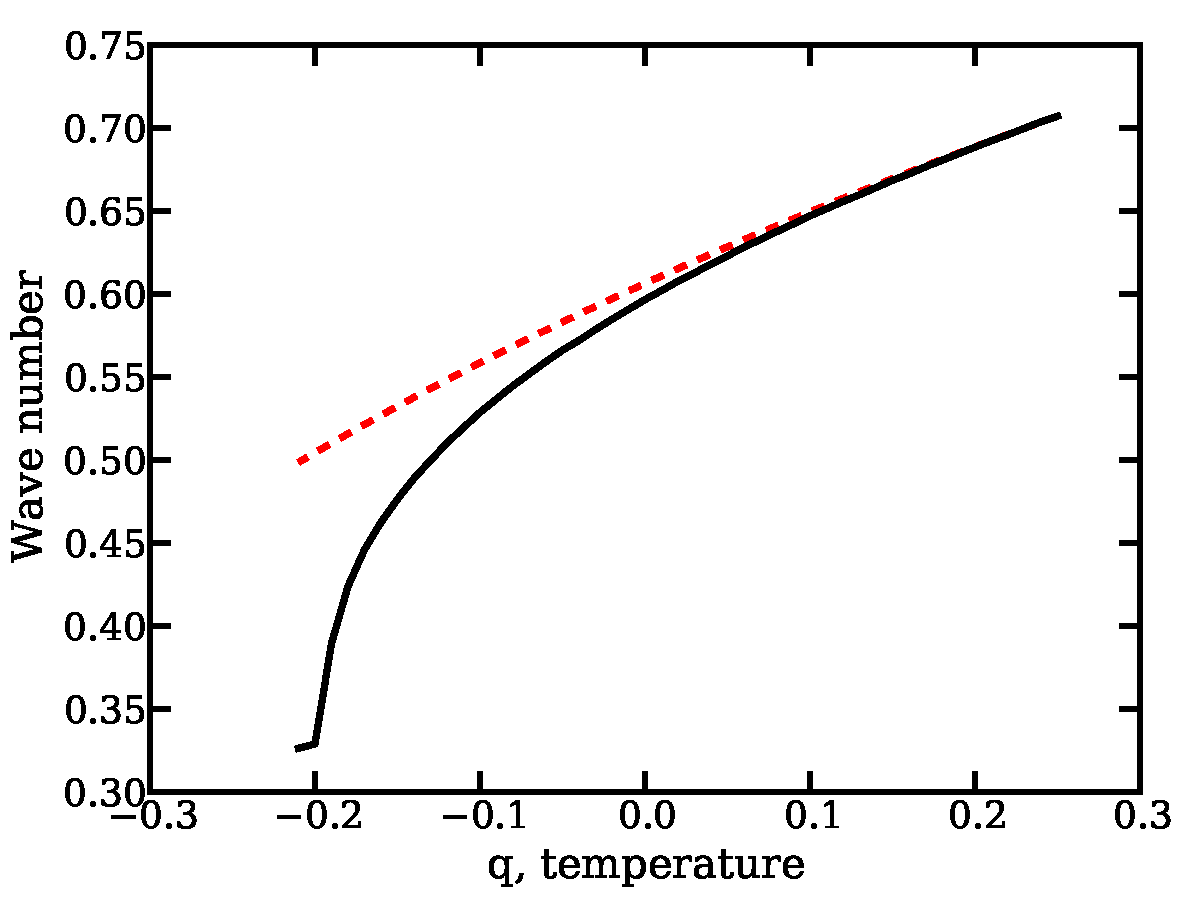
\includegraphics[width = 0.5\textwidth]{figs/gx3p_3-wn.pdf}
\caption{Результаты вычислений для волнового вектора при $g= -3.723$, $p_{icp}= -0.029$, $p_{cp}=-0.046$ ($g$ увеличено в 3 раза, $p$ уменьшено в 3 раза).}
\end{figure}

\begin{figure}\label{fig:px3-wn}
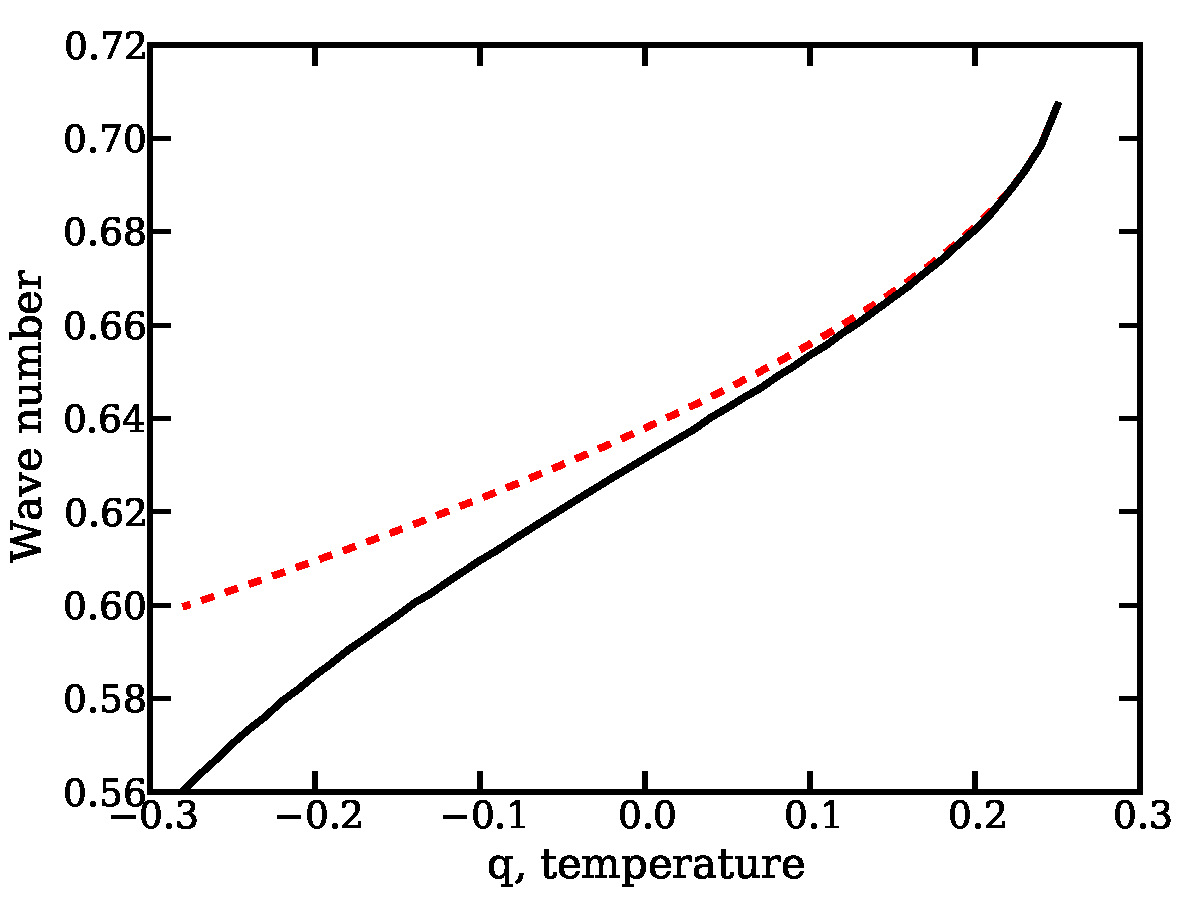
\includegraphics[width = 0.5\textwidth]{figs/px3-wn.pdf}
\caption{Результаты вычислений для волнового вектора при $g= -1.241$, $p_{icp}= -0.264$, $p_{cp}=-0.411$ ($p$ увеличено в 3 раза).}
\end{figure}

\begin{figure}\label{fig:g!3-wn}
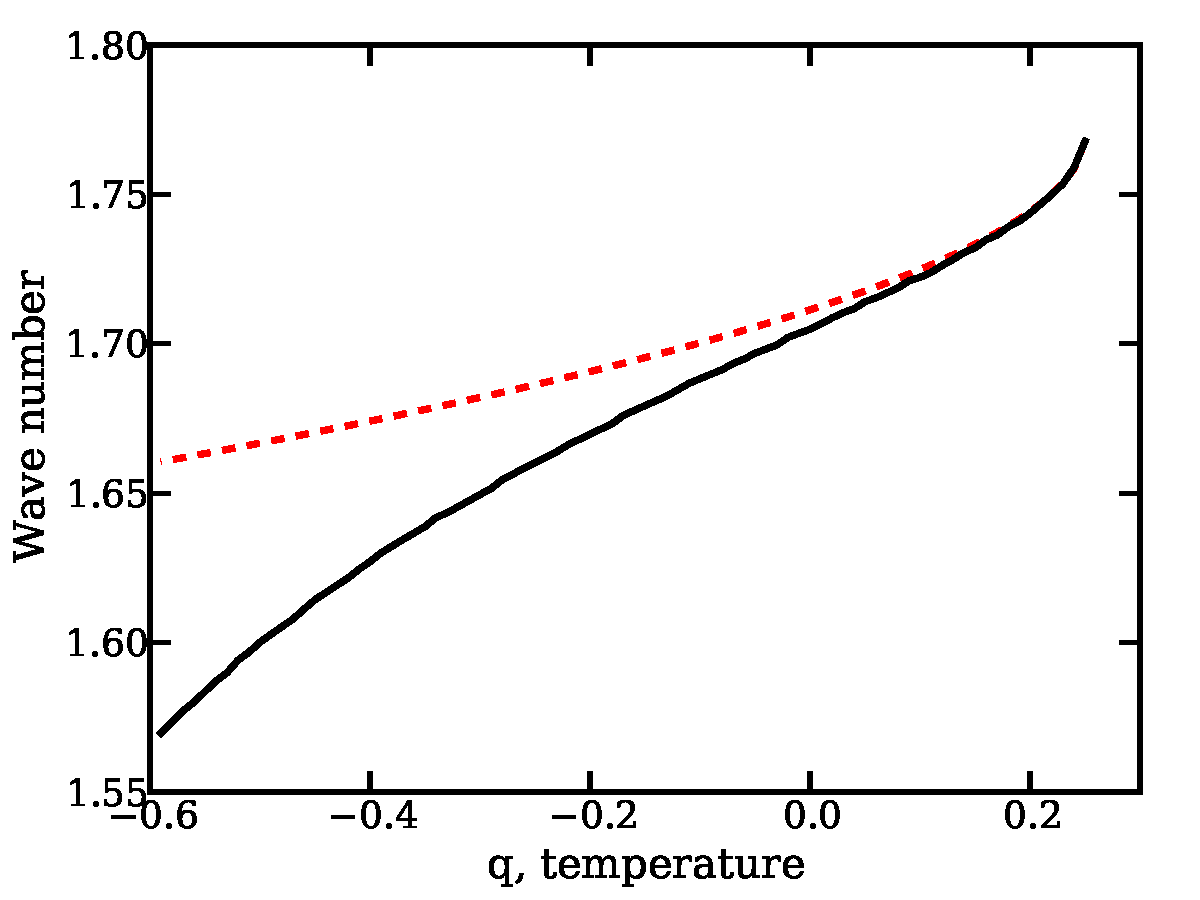
\includegraphics[width = 0.5\textwidth]{figs/g_3-wn.pdf}
\caption{Результаты вычислений для волнового вектора при $g= -0.414$, $p_{icp}= -0.088$, $p_{cp}=-0.137$ ($g$ уменьшено в 3 раза).}
\end{figure}

\begin{figure}\label{fig:gx3px3-cpt}
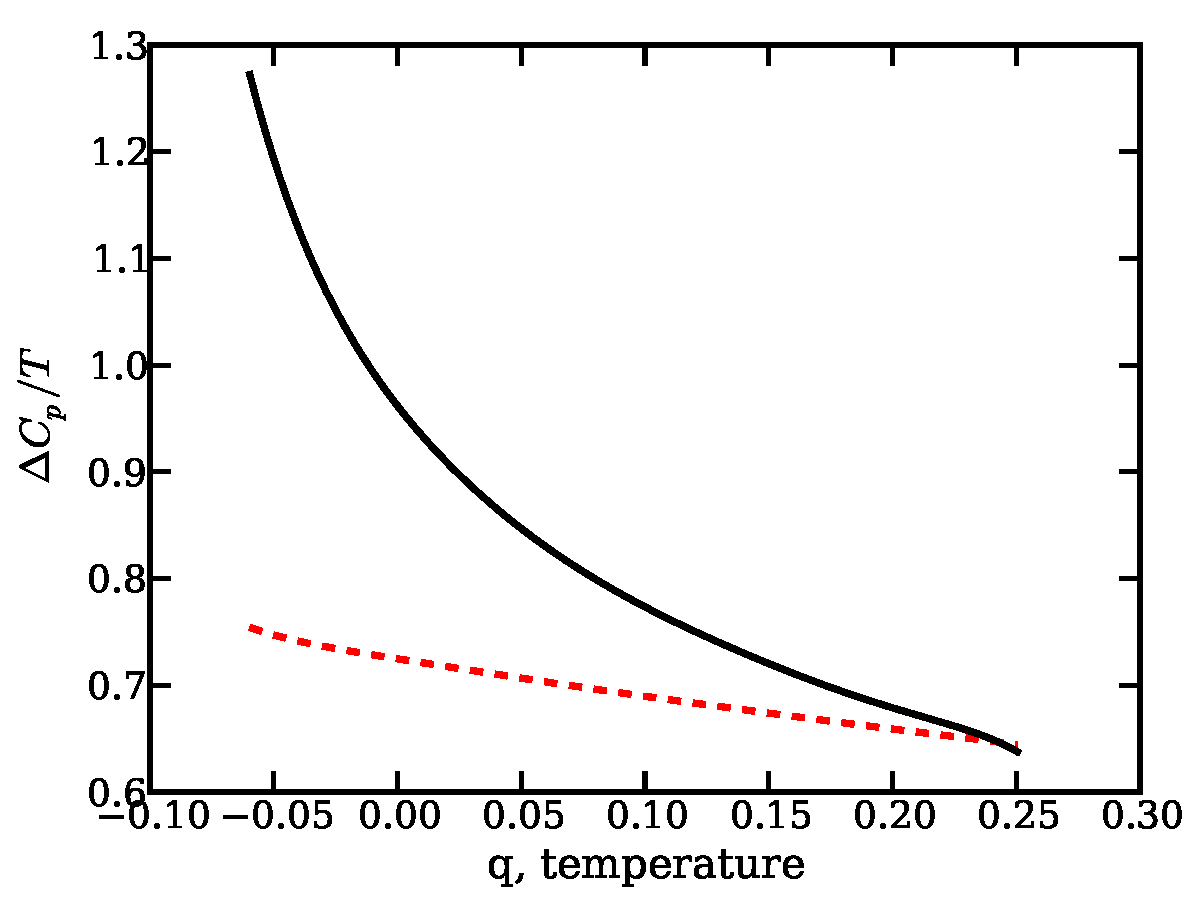
\includegraphics[width = 0.5\textwidth]{figs/gx3px3-cpt.pdf}
\caption{Результаты вычислений для отношения скачка теплоемкости к температуре при $g= -3.723$, $p_{icp}= -0.029$, $p_{cp}=-0.046$ ($g$ увеличено в 3 раза, $p$ увеличено в 3 раза)}
\end{figure}

\begin{figure}\label{fig:g!3-cpt}
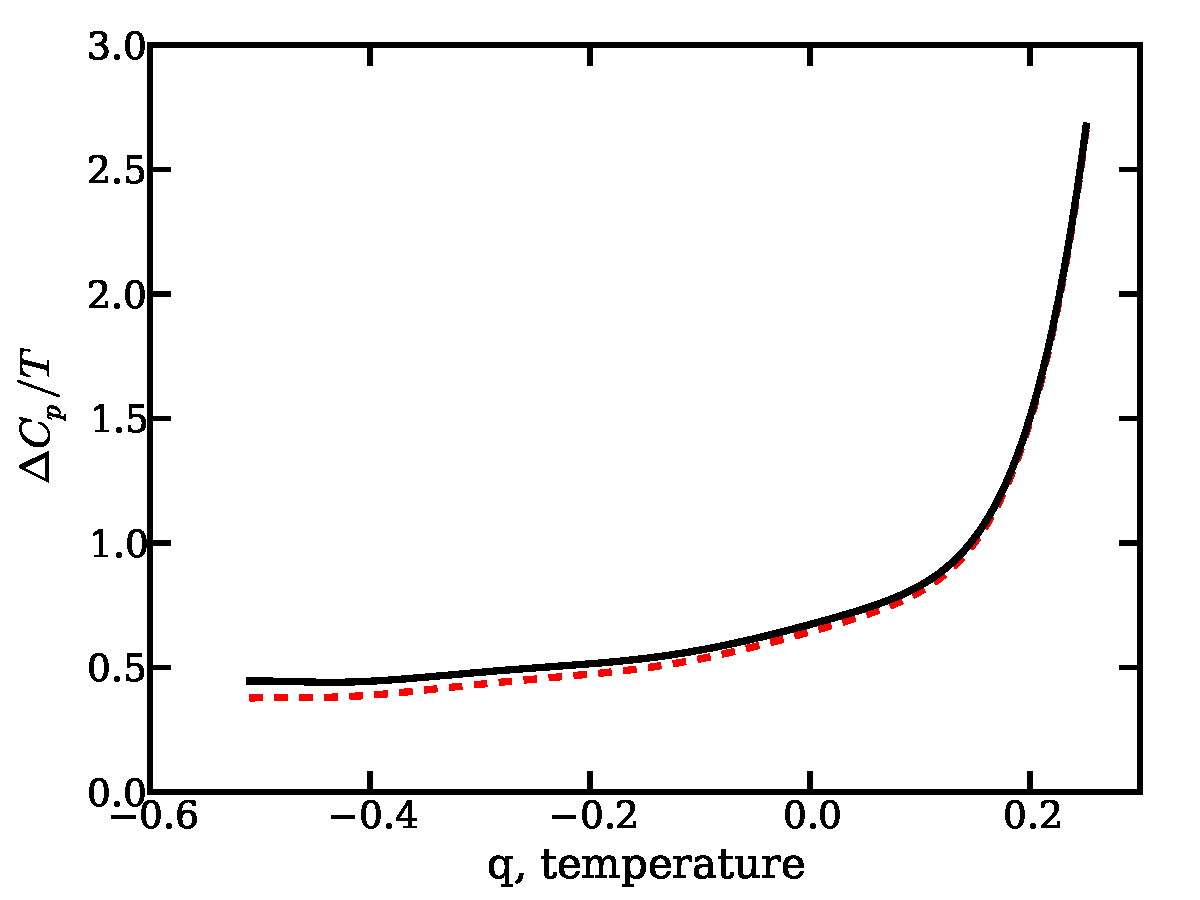
\includegraphics[width = 0.5\textwidth]{figs/g_3-cpt.pdf}
\caption{Результаты вычислений для отношения скачка теплоемкости к температуре при $g= -0.414$, $p_{icp}= -0.088$, $p_{cp}=-0.137$ ($g$ уменьшено в 3 раза).}
\end{figure}

\begin{figure}\label{fig:exp-wn}
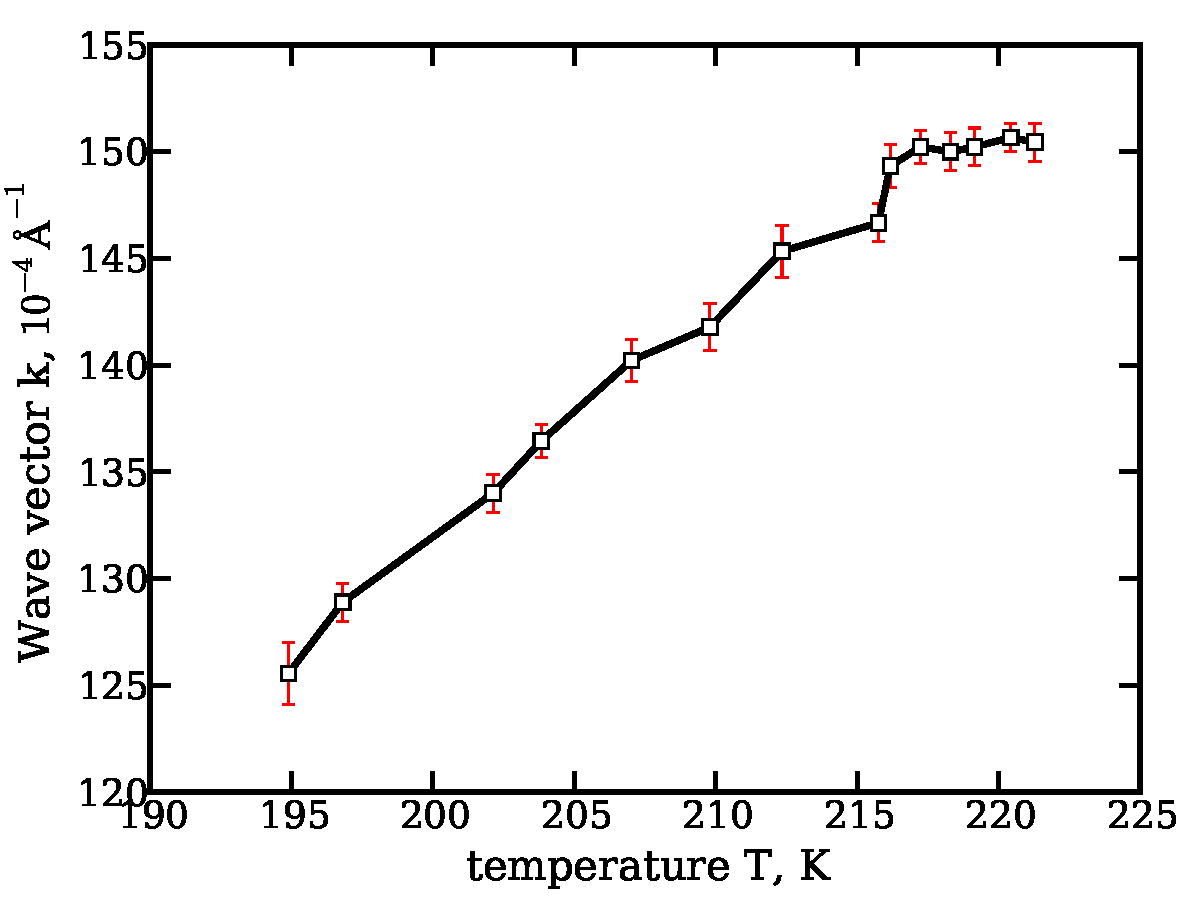
\includegraphics[width = 0.5\textwidth]{figs/exp-wn.pdf}
\caption{Экспериментальная кривая модуля волнового вектора модуляции ПП \protect\cite{Khoma1998}.}
\end{figure}

\begin{figure}\label{fig:exp-cp}
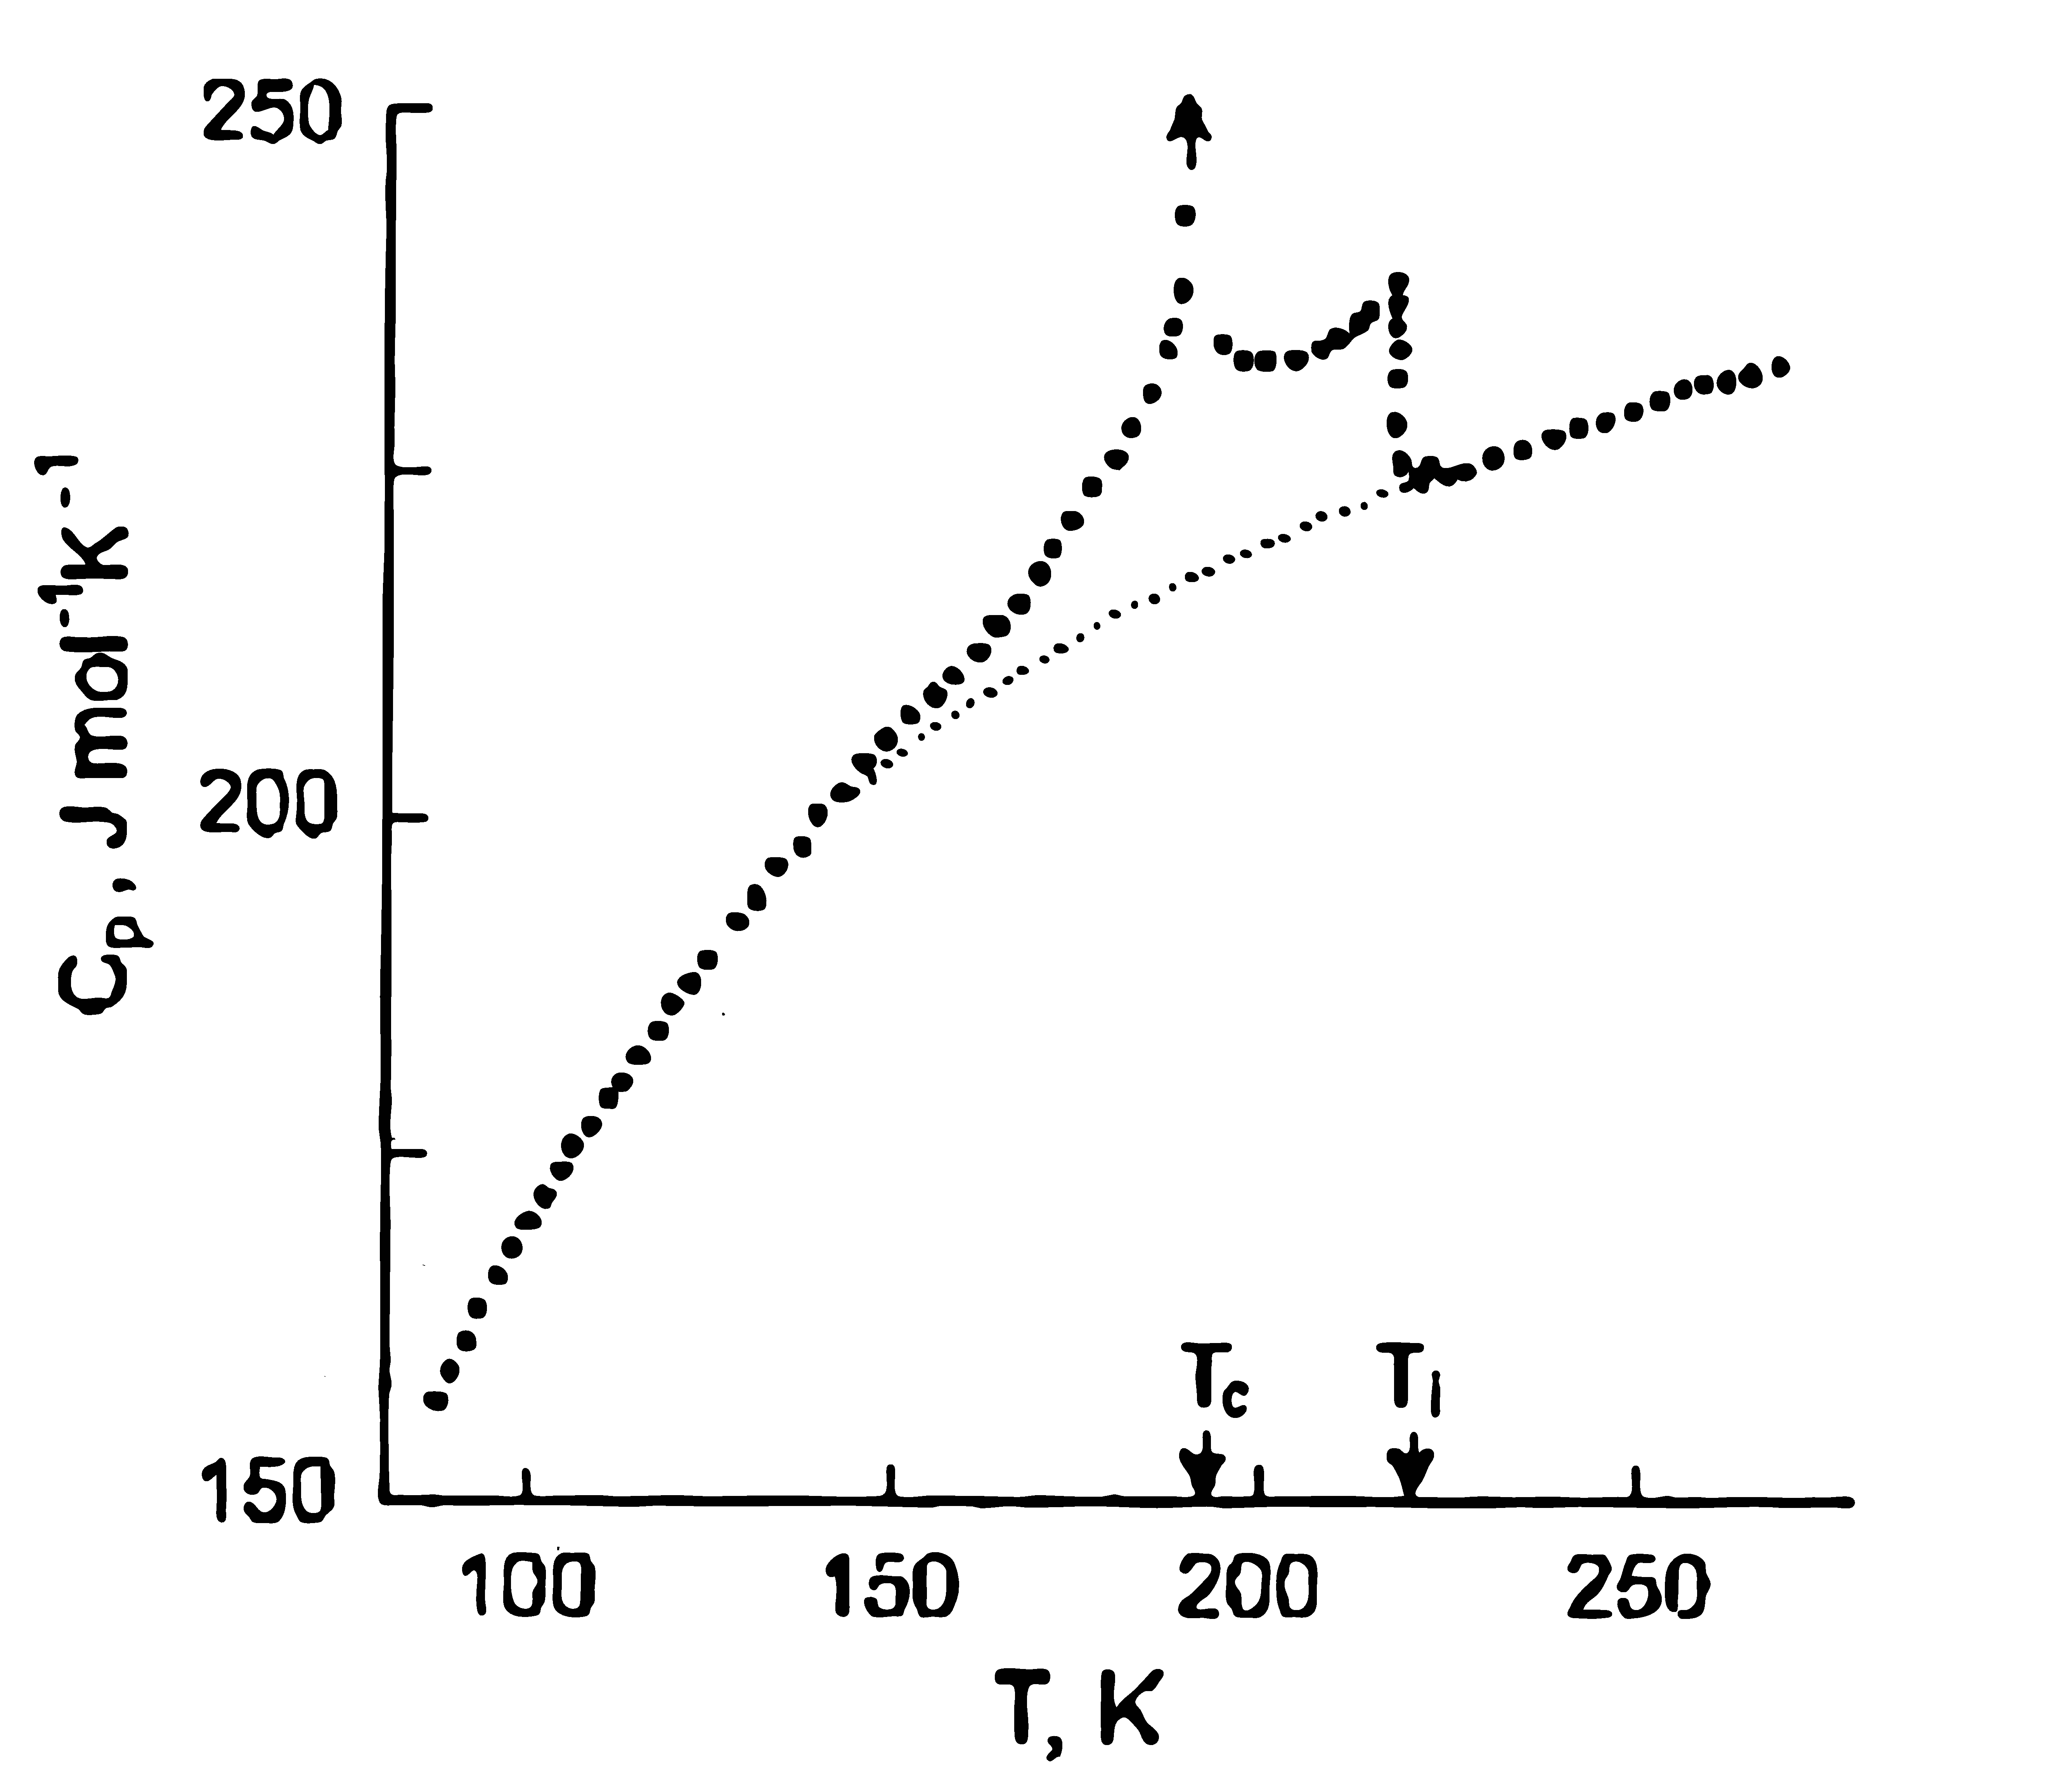
\includegraphics[width = 0.5\textwidth]{figs/exp-cp.pdf}
\caption{Экспериментальная кривая теплоемкости \protect\cite{Khoma1998}.}
\end{figure}